\documentclass[conference]{IEEEtran}

% =========================================================
% PACKAGES
% =========================================================
\usepackage[T1]{fontenc}
\usepackage{cite}
\usepackage{amsmath,amssymb}
\usepackage{graphicx}
\usepackage{booktabs}
\usepackage{array}
\usepackage{url}
\usepackage{microtype}
\usepackage{tikz}

\usetikzlibrary{
    arrows.meta,
    positioning,
    shapes.geometric,
    calc
}

% =========================================================
% TIKZ STYLES
% =========================================================
\tikzset{
    block/.style={
        rectangle,
        rounded corners=2pt,
        draw=black,
        align=center,
        minimum height=8mm,
        text width=1.65cm,
        font=\scriptsize,
        inner sep=3pt
    },
    flowblock/.style={
        rectangle,
        rounded corners=2pt,
        draw=black,
        align=center,
        minimum height=7mm,
        text width=2.6cm,
        font=\scriptsize,
        inner sep=3pt
    },
    decision/.style={
        diamond,
        draw=black,
        align=center,
        aspect=2.0,
        text width=1.2cm,
        font=\scriptsize,
        inner sep=1pt
    },
    arrow/.style={
        -{Stealth[length=1.7mm]},
        semithick
    }
}

% =========================================================
% TITLE
% =========================================================
\title{
Verification-Guided Q-Learning for Web Vulnerability Testing:
An Empirical Evaluation
}

\author{
\IEEEauthorblockN{Kevin Imanuel Setiawan}
\IEEEauthorblockA{
Program Studi Teknologi Informasi\\
Fakultas Informatika, Telkom University Surabaya\\
Surabaya, Indonesia\\
Email: your.email@example.com
}
}

\begin{document}

\maketitle

% =========================================================
% ABSTRACT
% =========================================================
\begin{abstract}
Automated web vulnerability testing can produce numerous
candidate findings, yet unusual application responses do not
necessarily indicate exploitable weaknesses. This study
evaluates a verification-guided Q-Learning prototype that
selects endpoint--payload actions against OWASP Juice Shop.
The agent observes HTTP responses, derives discrete state
features, and incorporates verification outcomes into reward
assignment. Its configured action space contains 120
endpoint--payload combinations, formed from eight endpoints
and 15 payloads per endpoint. During the reported run, the
agent executed 1,585 episodes over 142.55 seconds and recorded
14 verified vulnerable actions across five unique
endpoint--vulnerability-class pairs.
The recorded actions comprised six SQL injection actions,
five browser-verified cross-site scripting actions, and three
fuzzing or file-disclosure actions. The cumulative reward
was 3,783. In a separate detector benchmark, 13 true positives,
zero false positives, one false negative, and 60 true negatives
were observed among 74 labelled cases. Another 46 cases were
marked unknown and excluded from the evaluation. Recall and
F1-score were 0.929 and 0.963, respectively. The benchmark uses
a manually curated reference set and verification evidence
related to the prototype's own checks; it is not an independent
test on a new application. These results describe the configured
experiment and do not establish generalization or superiority
over existing scanners.
\end{abstract}

\begin{IEEEkeywords}
Automated penetration testing, reinforcement learning,
Q-Learning, web vulnerability testing, vulnerability
verification, OWASP Juice Shop
\end{IEEEkeywords}

% =========================================================
% 1. INTRODUCTION
% =========================================================
\section{Introduction}

Web applications process user input through numerous
interfaces, endpoints, and server-side components. Errors
in input handling or request processing can introduce
security weaknesses. Automated security testing can help
identify such weaknesses by sending test inputs and
examining the resulting application behavior. However,
an unusual response is not sufficient evidence that a
vulnerability can be exploited. Error messages, changes
in response length, and other observable differences may
also occur during normal application operation.

Reinforcement learning (RL) offers a framework for making
sequential decisions using feedback from an environment.
An agent selects an action, observes its consequences, and
updates its policy according to the reward received.
Q-Learning estimates the expected return of state--action
pairs and updates these estimates from observed transitions
\cite{sutton2018}.

Several studies have investigated learning-based approaches
to security testing. SQIRL applies reinforcement learning
to grey-box SQL injection detection \cite{sqirl2023}.
Other research has explored deep reinforcement learning
for vulnerability exploitation and autonomous penetration
testing \cite{almajali2024,li2025}. Recent review work
summarizes the development of reinforcement learning
approaches for automated penetration testing and discusses
their continuing challenges \cite{rlreview2026}. Comparisons
of autonomous penetration-testing agents further indicate
that their capabilities depend on the testing environment,
action design, and evaluation procedure \cite{sok2024}.

An important issue in automated testing is deciding when
an observation should be treated as a finding. A response
anomaly may indicate a candidate weakness, but the
conclusion should depend on evidence appropriate to the
testing category. This study therefore evaluates a
verification-guided Q-Learning prototype that separates
candidate signals from actions satisfying the implemented
verification criteria.

The study has three main contributions:

\begin{itemize}
    \item It presents a Q-Learning workflow in which
    verification evidence contributes to reward assignment.

    \item It reports empirical observations from a configured
    OWASP Juice Shop experiment, including recorded vulnerable
    actions, cumulative reward, and execution duration.

    \item It evaluates the prototype against a labelled
    reference set using recall and F1-score, and compares the
    evidence with prior RL-based security testing studies while
    excluding cases marked unknown.
\end{itemize}

The scope is limited to the configured application,
endpoint--payload combinations, and experimental procedures.
The results are not intended to establish performance
across arbitrary web applications.

% =========================================================
% 2. RELATED WORK
% =========================================================
\section{Related Work}

\subsection{Reinforcement Learning for Security Testing}

Reinforcement learning has been studied as a means of
automating security-related decisions. Rather than relying
entirely on a fixed sequence of tests, an agent can use
observations and rewards to update its action-selection
policy. SQIRL explores this approach for grey-box SQL
injection vulnerability detection \cite{sqirl2023}.

Deep reinforcement learning has also been investigated
for automated vulnerability exploitation. AlMajali
et al. studied a learning-based approach to selecting
actions during vulnerability exploitation \cite{almajali2024}.
Li et al. presented EPPTA, an approach based on partially
observable reinforcement learning for penetration-testing
applications \cite{li2025}. These studies provide related
examples of modelling security testing as a sequential
decision problem, although their methods and experimental
settings are not identical to the tabular Q-Learning
prototype evaluated here.

Liu et al. reviewed reinforcement learning approaches
for autonomous penetration testing and discussed
limitations that remain open for further research
\cite{rlreview2026}. Simon and Mees examined autonomous
penetration-testing agents from a comparative perspective,
highlighting the importance of evaluating agents in the
context of their capabilities and operating assumptions
\cite{sok2024}.

\subsection{Generalization and Evaluation}

Results obtained in one environment do not automatically
demonstrate that an agent will perform similarly in another.
Research into the generalizability of deep reinforcement
learning algorithms for automated vulnerability assessment
and penetration testing examines this issue across testing
conditions \cite{generalization2024}. Ghanem et al. studied
hierarchical reinforcement learning for automated
penetration testing in large networks, addressing the
challenge of organizing testing decisions in more complex
environments \cite{ghanem2023}.

These studies motivate reporting the experimental
configuration and limiting conclusions to the available
evidence. The present study focuses on a tabular Q-Learning
agent in a configured OWASP Juice Shop environment.
It does not claim that the learned policy generalizes
to applications not included in the experiment.

\subsection{Web Vulnerability Verification}

Automated testing systems may encounter response anomalies
that are not sufficient to confirm a vulnerability.
The OWASP Web Security Testing Guide provides structured
guidance for examining web application security, including
input validation and client-side testing \cite{owaspwstg}.
Following this general principle, the prototype distinguishes
between a candidate signal and a finding that satisfies
its configured verification criteria.

For XSS candidates, the system uses browser-based checks
implemented with Playwright \cite{playwright}. These checks
provide additional observations beyond the initial HTTP
response. Their effectiveness, however, remains bounded
by the test cases and browser interactions implemented
in the prototype.

% =========================================================
% 3. METHODOLOGY
% =========================================================
\section{Methodology}

\subsection{Experimental Environment}

The experiment used OWASP Juice Shop version 20.2.0
in a local environment. OWASP Juice Shop is an intentionally
insecure web application designed for security education
and testing \cite{juiceshop}.

The prototype uses a configured set of eight endpoints
and 15 payloads per endpoint. The Q-Learning agent selects
endpoint--payload actions, submits requests to the target,
observes the resulting HTTP responses, and updates its
state--action estimates according to the reward assigned
to each outcome.

The evaluation describes the reported configuration.
Different application versions, endpoints, payloads, or
verification rules may produce different results.

\subsection{HTTP API and Endpoint Coverage}

The target is accessed through HTTP routes exposed by Juice
Shop. The configured surface includes REST API routes and the
\texttt{/ftp/} file-serving route. For each selected action,
the client inserts the payload into the route's configured
query parameter, appends it to the route when the parameter
is a path, or sends it in a JSON body for POST and PUT
requests. The response status, body length, content type,
and response time provide observations for state construction.
Table~\ref{tab:api-endpoints} lists the eight routes used by
the agent.

\begin{table}[!t]
\caption{HTTP Routes Used in the Experiment}
\label{tab:api-endpoints}
\centering
\footnotesize
\setlength{\tabcolsep}{3pt}
\begin{tabular}{c p{0.41\columnwidth} p{0.43\columnwidth}}
\toprule
\textbf{Idx.} & \textbf{Method and route} & \textbf{Role in the experiment}\\
\midrule
0 & GET \url{/rest/products/search?q=} & Product search; SQLi and search-page XSS checks\\
1 & GET \url{/ftp/} + path & File-serving route; path and extension-bypass checks\\
2 & GET \url{/rest/products/1/reviews?id=} & Review retrieval; plain-surface control\\
3 & GET \url{/rest/track-order/} + path & Order tracking; browser-based XSS checks on the result page\\
4 & POST \url{/rest/user/login} & Login request with a JSON body; SQLi checks\\
5 & PUT \url{/rest/products/1/reviews} & Review submission with a JSON body; plain-surface control\\
6 & POST \url{/api/Feedbacks} & Feedback JSON body; requires CAPTCHA fields\\
7 & GET \url{/api/Challenges?q=} & Challenge API; plain-surface control\\
\bottomrule
\end{tabular}
\end{table}
\setlength{\tabcolsep}{6pt}

The feedback route requires an additional GET request to
\url{/rest/captcha}; its returned answer and identifier are
included with the feedback JSON body, together with the
configured defaults \texttt{rating=1} and \texttt{UserId=1}.
Before training,
the prototype sends a benign \texttt{hello} probe to each of
the eight routes to establish endpoint-specific response
baselines. The two XSS-capable routes are also checked through
their corresponding Juice Shop single-page application (SPA)
pages, because an HTTP response containing a vector does not
by itself show that the browser executed it.
The configured \texttt{sql}, \texttt{file}, and \texttt{plain}
surface labels restrict which detector checks apply to each
route. They are source-informed metadata about possible input
sinks, not preassigned vulnerability findings; each candidate
must still pass the verification workflow.

\subsection{Action Space}

Let $\mathcal{E}$ denote the configured endpoint set and
$\mathcal{P}$ the configured payload set. The action space
is defined as

\begin{equation}
\mathcal{A} = \mathcal{E} \times \mathcal{P}.
\label{eq:actionspace}
\end{equation}

With eight endpoints and 15 payloads per endpoint, the
number of configured endpoint--payload combinations is

\begin{equation}
|\mathcal{A}| = |\mathcal{E}| \times |\mathcal{P}|
= 8 \times 15 = 120.
\label{eq:actioncount}
\end{equation}

An action corresponds to submitting a configured payload
to a selected endpoint. The observed response is then
processed to construct the next state.

\subsection{State Representation}

The prototype represents observations using eight features:

\begin{equation}
\begin{split}
s_t = (&\text{status\_cat},
\text{length\_cat},
\text{err\_flag},
\text{refl\_flag},\\
&\text{vuln\_ind},
\text{ep\_idx},
\text{resp\_time\_cat},
\text{content\_cat}).
\end{split}
\label{eq:state}
\end{equation}

These features represent the HTTP status category,
response-length category, error flag, reflection flag,
vulnerability indicator, endpoint index, response-time
category, and content category.

Response-length deviation is measured relative to the
configured baseline for an endpoint. A deviation greater
than 15\% is treated as a significant change by the
prototype. Response time is classified as fast when it
is below 0.5 seconds, medium from 0.5 to 2.0 seconds,
and slow when it exceeds 2.0 seconds.

The resulting representation converts selected response
characteristics into discrete features. Its coverage
depends on the features and thresholds implemented in
the prototype.

\subsection{Q-Learning Update}

The agent updates the value of a state--action pair using
the observed reward and the maximum estimated value of
the next state. The update rule is

\begin{equation}
\footnotesize
Q(s_t,a_t) \leftarrow Q(s_t,a_t) + \alpha \big[ r_t + \gamma \max_{a'} Q(s_{t+1},a') - Q(s_t,a_t) \big],
\label{eq:ql}
\end{equation}

where $s_t$ is the current state, $a_t$ is the selected
action, $r_t$ is the observed reward, $s_{t+1}$ is the
next state, $\alpha$ is the learning rate, and $\gamma$
is the discount factor \cite{sutton2018}.

The reported configuration uses $\alpha=0.1$ and
$\gamma=0.9$. An $\epsilon$-greedy policy controls the
balance between exploration and exploitation; $\epsilon$
starts at 1.0, decays by 0.90 per episode, and has a minimum
of 0.1.
Training always uses the complete budget of 1,585 episodes.
Only actions already verified as vulnerable are masked from
future selection; unsuccessful actions remain available, and
the run does not stop early.

\subsection{Verification-Guided Reward Assignment}

The prototype assigns rewards according to the observed
outcome and verification status. The configured reward
values are listed in Table~\ref{tab:rewards}.

\begin{table}[!t]
\caption{Configured Reward Values}
\label{tab:rewards}
\centering
\footnotesize
\begin{tabular}{p{0.66\columnwidth}r}
\toprule
\textbf{Outcome} & \textbf{Reward}\\
\midrule
Verified vulnerable action & $+50$\\
Unverified response anomaly & $+10$\\
Normal response & $-1$\\
Connection failure or timeout & $-5$\\
\bottomrule
\end{tabular}
\end{table}

A candidate anomaly is not automatically treated as a
verified finding. For SQLi and fuzzing/file-disclosure
candidates, the prototype sends a benign \texttt{hello}
control and, when it differs from the tested input, a
neutralized payload control. A candidate is retained only
when neither control reproduces the same vulnerability class;
connection errors are inconclusive. For XSS, a headless
Chromium browser loads the corresponding SPA page with an
instrumented vector, and the finding is accepted only when
the execution canary runs in the DOM while any distinct
neutralized control does not. HTTP reflection alone is
insufficient. These category-specific checks determine
whether the verified-finding reward is assigned.

The listed values are base category rewards; a response-length
bonus of $+0$, $+0$, $+5$, or $+10$ is added according to the
configured length category. The reward values are configuration
parameters rather than values established through a
reward-sensitivity study. Consequently, the reported experiment
does not demonstrate that these values are optimal.

\subsection{System Architecture}

Fig.~\ref{fig:architecture} illustrates the interaction
between the Q-Learning agent, the target application,
state construction, and verification stage.

\begin{figure}[!t]
\centering
\resizebox{\columnwidth}{!}{%
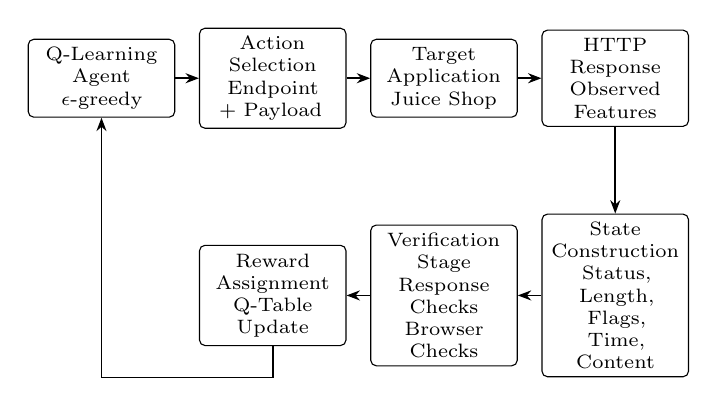
\begin{tikzpicture}[
    node distance=4mm and 3mm
]
\node[block] (agent) {
    Q-Learning\\Agent\\
    $\epsilon$-greedy
};

\node[block, right=of agent] (action) {
    Action Selection\\
    Endpoint + Payload
};

\node[block, right=of action] (target) {
    Target Application\\
    Juice Shop
};

\node[block, right=of target] (response) {
    HTTP Response\\
    Observed Features
};

\node[block, below=11mm of response] (state) {
    State Construction\\
    Status, Length, Flags,\\
    Time, Content
};

\node[block, left=of state] (verify) {
    Verification Stage\\
    Response Checks\\
    Browser Checks
};

\node[block, left=of verify] (reward) {
    Reward Assignment\\
    Q-Table Update
};

\draw[arrow] (agent) -- (action);
\draw[arrow] (action) -- (target);
\draw[arrow] (target) -- (response);
\draw[arrow] (response) -- (state);
\draw[arrow] (state) -- (verify);
\draw[arrow] (verify) -- (reward);

\draw[arrow]
    (reward.south) -- ++(0,-4mm)
    -| (agent.south);

\end{tikzpicture}%
}
\caption{Workflow of the verification-guided Q-Learning prototype.}
\label{fig:architecture}
\end{figure}

The agent first selects an endpoint--payload combination.
The target application returns a response, which is
converted into state features. The verification stage
then provides evidence used by reward assignment and
the Q-table update.

\subsection{Verification Workflow}

The verification workflow separates candidate signals
from actions satisfying the configured criteria. As
shown in Fig.~\ref{fig:verification}, an observation
without a candidate signal is recorded as an ordinary
response. A candidate signal proceeds to the relevant
verification checks.

\begin{figure}[!t]
\centering
\resizebox{0.9\columnwidth}{!}{%
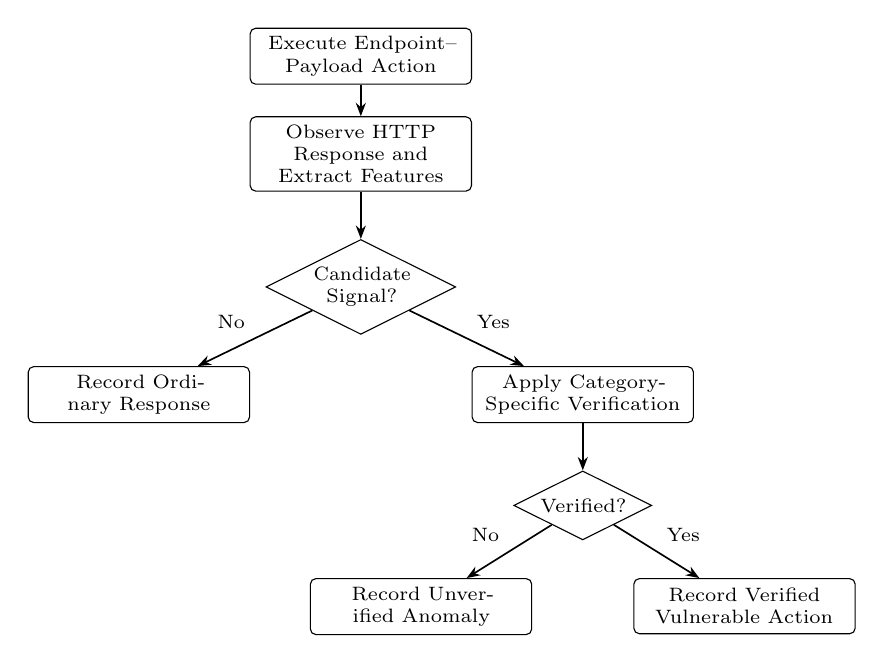
\begin{tikzpicture}[
    node distance=4mm
]
\node[flowblock] (execute) {
    Execute Endpoint--Payload Action
};

\node[flowblock, below=of execute] (observe) {
    Observe HTTP Response and Extract Features
};

\node[decision, below=6mm of observe] (candidate) {
    Candidate\\Signal?
};

\node[flowblock, below left=7mm and 8mm of candidate] (ordinary) {
    Record Ordinary Response
};

\node[flowblock, below right=7mm and 8mm of candidate] (checks) {
    Apply Category-Specific Verification
};

\node[decision, below=6mm of checks] (verified) {
    Verified?
};

\node[flowblock, below left=7mm and 2mm of verified] (unverified) {
    Record Unverified Anomaly
};

\node[flowblock, below right=7mm and 2mm of verified] (finding) {
    Record Verified Vulnerable Action
};

\draw[arrow] (execute) -- (observe);
\draw[arrow] (observe) -- (candidate);

\draw[arrow]
    (candidate) -- node[above left,font=\scriptsize] {No}
    (ordinary);

\draw[arrow]
    (candidate) -- node[above right,font=\scriptsize] {Yes}
    (checks);

\draw[arrow] (checks) -- (verified);

\draw[arrow]
    (verified) -- node[above left,font=\scriptsize] {No}
    (unverified);

\draw[arrow]
    (verified) -- node[above right,font=\scriptsize] {Yes}
    (finding);

\end{tikzpicture}%
}
\caption{Verification process for candidate anomalies.}
\label{fig:verification}
\end{figure}

Candidates that do not satisfy the configured checks
are recorded as unverified anomalies rather than verified
vulnerable actions. Candidates that satisfy the checks
are recorded as verified vulnerable actions. This
workflow describes the implemented criteria and should
not be interpreted as exhaustive verification of every
possible vulnerability.

\subsection{Evaluation Metrics}

The reference-set evaluation uses true positives (TP),
false positives (FP), false negatives (FN), and true
negatives (TN). We report recall, which measures the share
of labelled vulnerable actions detected, and F1-score, which
combines recall with precision. Cases marked unknown are
excluded, so these results describe only the labelled subset.

\begin{equation}
\mathrm{Recall} = \frac{TP}{TP+FN}.
\label{eq:recall}
\end{equation}

\begin{equation}
\mathrm{F1} =
2\frac{\mathrm{Precision}\times\mathrm{Recall}}
{\mathrm{Precision}+\mathrm{Recall}}.
\label{eq:f1}
\end{equation}

% =========================================================
% 4. RESULTS AND DISCUSSION
% =========================================================
\section{Results and Discussion}

\subsection{Summary of the Q-Learning Run}

Table~\ref{tab:run-summary} summarizes the recorded
Q-Learning run. The values represent the reported
experiment rather than averages across independent runs.
Run metrics are in-sample observations from the training
episodes; the separate detector benchmark evaluates the
response analyzer against the curated reference set.

\begin{table}[!t]
\caption{Summary of the Reported Q-Learning Run}
\label{tab:run-summary}
\centering
\footnotesize
\begin{tabular}{p{0.66\columnwidth}r}
\toprule
\textbf{Measure} & \textbf{Value}\\
\midrule
Episodes executed & 1,585\\
Endpoint--payload combinations & 120\\
Verified vulnerable actions & 14\\
Unique endpoint--class pairs & 5\\
SQL injection actions & 6\\
Browser-verified XSS actions & 5\\
Fuzzing/file-disclosure actions & 3\\
Cumulative reward & 3,783\\
Total request interactions, including baselines and verification & 1,639\\
Training duration & 142.55 s\\
\bottomrule
\end{tabular}
\end{table}

The run executed all 1,585 budgeted episodes and recorded 14
verified vulnerable actions across five unique
endpoint--vulnerability-class pairs. The action count
consisted of six SQL injection actions, five browser-verified
XSS actions, and three fuzzing or file-disclosure actions.
The 1,585 episodes count the agent's selected actions. Eight
baseline probes and 46 verification requests were additional,
bringing the recorded request interactions to 1,639.

The 14 actions represent verified endpoint--payload
combinations, whereas the five pairs count distinct
endpoint and vulnerability-class combinations. They should
not be interpreted as 14 independently confirmed root-cause
vulnerabilities.

The cumulative reward was 3,783. This figure reflects
the sequence of outcomes and the reward values configured
in the prototype. It is not a direct measure of
vulnerability severity or a standalone measure of testing
quality.

\subsection{Observed Discovery Timeline}

The first recorded finding occurred at episode 1, while
all 14 recorded actions had been discovered by episode
787. This describes the discovery sequence observed in
the reported run.

The timeline does not demonstrate that another run
would discover findings at the same rate. Discovery
behavior can depend on the initial state, exploration
policy, configured action space, target responses, and
verification criteria. Repeated independent runs would
be needed to assess variability in the observed timeline.

\subsection{Reference-Set Evaluation}

The separate detector benchmark applies the response
analyzer to all 120 configured endpoint--payload actions
without an RL agent and compares its outputs with the
manually curated labels. Table~\ref{tab:benchmark-results}
reports the confusion counts and the two selected metrics.
The labelled subset contains 74 cases; 46 cases are marked
unknown and excluded.

\begin{table}[!t]
\caption{Detector Benchmark on the Labelled Reference Set}
\label{tab:benchmark-results}
\centering
\footnotesize
\begin{tabular}{lc}
\toprule
\textbf{Measure} & \textbf{Value}\\
\midrule
True positives (TP) & 13\\
False positives (FP) & 0\\
False negatives (FN) & 1\\
True negatives (TN) & 60\\
Unknown cases, excluded & 46\\
Recall & 0.929\\
F1-score & 0.963\\
\bottomrule
\end{tabular}
\end{table}

The benchmark produced a recall of 0.929 and an F1-score of
0.963. No false positives were recorded among the 60 labelled
negative actions. The false-negative count was one.

These results must be interpreted in relation to the
reference set. The 46 unknown cases were not included
in the calculations and should not be considered correctly
classified negative cases.

The manual reference checks use evidence related to the
prototype's own control-differential and browser-execution
checks. Agreement between the detector and labels is
therefore not fully independent. The results demonstrate
consistency with this curated reference set, not perfect
detection or generalization to unseen applications.

\subsection{Comparison with Prior Work}

Table~\ref{tab:prior-comparison} places the observed results
alongside prior reinforcement-learning studies. The reported
values are included as evidence of what each study measured;
they do not form a head-to-head ranking because the targets,
access models, action spaces, and success criteria differ.

\begin{table*}[!t]
\caption{Contextual Comparison with Prior RL-Based Security Testing}
\label{tab:prior-comparison}
\centering
\scriptsize
\setlength{\tabcolsep}{3pt}
\begin{tabular}{p{0.95in} p{3.15in} p{2.90in}}
\toprule
\textbf{Study} & \textbf{Setting and reported evidence} & \textbf{Relation to this study}\\
\midrule
SQIRL \cite{sqirl2023} & Deep RL with grey-box feedback for SQL injection. It found all vulnerabilities in its SQLi microbenchmark using substantially fewer requests than most compared scanners; on 14 production applications it reported 33 vulnerabilities and zero false positives. & SQIRL evaluates SQLi across production applications and uses database-side feedback. This study uses a fixed Juice Shop endpoint--payload set and includes SQLi, browser-verified XSS, and file/fuzzing checks.\\
AlMajali et al. \cite{almajali2024} & Deep RL and Q-table agents were evaluated on two Metasploitable exploitation scenarios. The best reported reverse-shell success rates for DRL versus Q-table were 96.6\% versus 88.4\% and 73.6\% versus 71.2\%. & Their outcome is successful exploitation and reverse-shell establishment, not vulnerability-detector recall. The success rates are not directly comparable with this study's reference-set metrics.\\
This study & Tabular Q-Learning tested 120 actions across eight Juice Shop routes. The training run recorded 14 verified actions across five endpoint--class pairs. The separate detector benchmark reported 13 TP, 1 FN, 0 FP, and 60 TN; recall was 0.929 and F1-score was 0.963, with 46 unknown cases excluded. & This experiment includes multiple web vulnerability categories and explicit response controls and browser checks. Its scope is one application and a human-configured endpoint--payload set; the benchmark labels also use evidence related to the implemented checks.\\
\bottomrule
\end{tabular}
\end{table*}
\setlength{\tabcolsep}{6pt}

The SoK comparison by Simon and Mees notes that differences
in environment modelling, scenarios, algorithms, and methods
make performance conclusions across autonomous penetration
testing agents difficult to draw \cite{sok2024}. Accordingly,
the prior results provide context for the task and evaluation
scope, rather than a numerical claim that one approach
outperforms another.

\subsection{Role of Verification}

Verification is intended to reduce the risk of treating
every response anomaly as a confirmed vulnerability.
This distinction is particularly relevant when observable
response changes may have explanations other than
successful exploitation.

The reported run included five browser-verified XSS
actions. Browser checks provide observations beyond the
initial HTTP response, but their conclusions remain
limited to the checks and conditions implemented in
the prototype.

The reference-set evaluation also contained one false
negative. The available aggregate results do not establish
the cause of this case. Further examination of the
corresponding logs and verification trace would be
required before assigning a specific explanation.

\subsection{Limitations}

The results should be considered alongside several
limitations.

First, the experiment was performed against a configured
local instance of OWASP Juice Shop. It does not establish
that the same results would be obtained on other
applications or application versions.

Second, the action space was restricted to eight
configured endpoints and 15 payloads per endpoint.
Potential weaknesses outside this space may not be
observed by the agent.

Third, the state representation converts selected response
features into discrete categories. Consequently, response
behaviors not captured by these features may not be
adequately distinguished.

Fourth, the reward values were configured for the
prototype. No sensitivity analysis was conducted to
establish whether alternative values would produce
different results.

Fifth, the reported run does not establish statistical
reliability across repeated independent trials.
Additional experiments are required to characterize
run-to-run variability.

Finally, the payload list and surface gating were specified
by the researchers with prior knowledge of the Juice Shop
source structure. This human prior constrains the action
space; the agent still selects among the configured actions,
and findings must pass the implemented verification checks.
The reference-set metrics also exclude unknown cases, and
the manual labels use evidence related to the prototype's
verification procedure.

% =========================================================
% 5. CONCLUSION
% =========================================================
\section{Conclusion}

This study evaluated a verification-guided Q-Learning
prototype for web vulnerability testing against OWASP
Juice Shop. In the reported run, the agent executed
1,585 episodes using an action space of 120
endpoint--payload combinations and completed execution
in 142.55 seconds. The system recorded 14 verified
actions across five unique endpoint--vulnerability-class pairs,
including six SQL injection actions, five browser-verified
XSS actions, and three fuzzing or file-disclosure actions.

The separate detector benchmark reported recall of 0.929
and F1-score of 0.963 on the labelled subset, with 46 unknown
actions excluded. Because the manual reference checks use
evidence related to the prototype's verification procedure,
these values show consistency with the curated reference set
rather than independent generalization. Comparisons with
prior studies are contextual because their target systems and
success criteria differ.

Future work should examine repeated independent runs,
test the sensitivity of the results to reward and
state-discretization parameters, and evaluate the approach
against additional applications using explicitly matched
baseline configurations and independently defined labels.

% =========================================================
% ACKNOWLEDGMENT
% =========================================================
\section*{Acknowledgment}

The author thanks the academic supervisors and individuals
who provided feedback during the development and evaluation
of this research.

% =========================================================
% REFERENCES
% =========================================================
\begin{thebibliography}{99}

\bibitem{sqirl2023}
A. Al Wahaibi, S. Foley, and S. Maffeis,
``SQIRL: Grey-Box Detection of SQL Injection Vulnerabilities
Using Reinforcement Learning,''
in \textit{Proceedings of the 32nd USENIX Security Symposium},
2023, pp. 6097--6114.

\bibitem{rlreview2026}
J. Liu et al.,
``Autonomous penetration testing using reinforcement learning:
A review and perspectives,''
\textit{Expert Systems with Applications},
vol. 300, Art. no. 130219, 2026,
doi: 10.1016/j.eswa.2025.130219.

\bibitem{sok2024}
M. Simon and S. Mees,
``SoK: A Comparison of Autonomous Penetration Testing Agents,''
in \textit{Proceedings of the 19th International Conference on
Availability, Reliability and Security (ARES)}, 2024,
doi: 10.1145/3664476.3664484.

\bibitem{sutton2018}
R. S. Sutton and A. G. Barto,
\textit{Reinforcement Learning: An Introduction},
2nd ed. Cambridge, MA, USA: MIT Press, 2018.

\bibitem{juiceshop}
OWASP Foundation,
``OWASP Juice Shop.''
[Online]. Available:
\url{https://owasp.org/www-project-juice-shop/}

\bibitem{owaspwstg}
OWASP Foundation,
``Web Security Testing Guide.''
[Online]. Available:
\url{https://owasp.org/www-project-web-security-testing-guide/}

\bibitem{playwright}
Microsoft,
``Playwright Documentation.''
[Online]. Available:
\url{https://playwright.dev/docs/intro}

\bibitem{almajali2024}
A. AlMajali, L. Al-Abed, K. M. A. Yousef,
B. J. Mohd, Z. Samamah, and A. Abu Shhadeh,
``Automated Vulnerability Exploitation Using Deep Reinforcement
Learning,''
\textit{Applied Sciences},
vol. 14, no. 20, Art. no. 9331, 2024,
doi: 10.3390/app14209331.

\bibitem{li2025}
Z. Li et al.,
``EPPTA: Efficient partially observable reinforcement learning
agent for penetration testing applications,''
\textit{Engineering Reports},
vol. 7, no. 1, Art. no. e12818, 2025,
doi: 10.1002/eng2.12818.

\bibitem{generalization2024}
``Assessing generalizability of Deep Reinforcement Learning
algorithms for Automated Vulnerability Assessment and
Penetration Testing,''
\textit{Array}, vol. 24, Art. no. 100365, 2024,
doi: 10.1016/j.array.2024.100365.

\bibitem{ghanem2023}
M. C. Ghanem, T. M. Chen, and E. G. Nepomuceno,
``Hierarchical reinforcement learning for efficient and effective
automated penetration testing of large networks,''
\textit{Journal of Intelligent Information Systems},
vol. 60, pp. 281--303, 2023,
doi: 10.1007/s10844-022-00738-0.

\end{thebibliography}

\end{document}
